\setcounter{dang}{0}
\newpage
\section{PHƯƠNG TRÌNH MẶT CẦU}
\subsection{LÝ THUYẾT CẦN NHỚ}
\subsubsection{Định nghĩa}
\begin{itemize}
	\immini{	\item [\iconCH] Trong không gian, tập hợp tất cả các điểm $M$  cách điểm $I$ cố định một khoảng không đổi $r$ $(r>0)$  cho trước được gọi là mặt cầu tâm $I$ bán kính $R$. Kí hiệu $S(I;r)$ hay viết tắt là $(S)$. Vậy $S(I;R)=\{M|IM=r\}.$
		\item [\iconCH] Nhận xét: 
		\begin{itemize}
			\item Nếu $IM=r$ thì $M$ nằm trên mặt cầu.
			\item 	Nếu $IM<r$ thì $M$ nằm trong mặt cầu.
			\item 	Nếu $I M>r$ thì $M$ nằm ngoài mặt cầu.
		\end{itemize}
	}{
		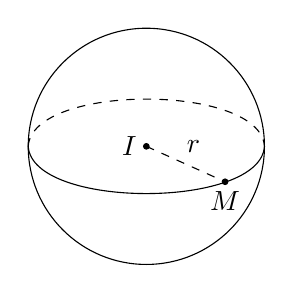
\begin{tikzpicture}
			\draw[fill=black] (0,0) circle(1pt) node[left]{$I$};
			\draw (0,0) circle(1.5);
			\draw (-1.5,0)..controls (-1.45,-0.8) and (1.45,-0.8)..(1.5,0);
			\draw[dashed] (-1.5,0)..controls (-1.45,0.8) and (1.45,0.8)..(1.5,0);
			\draw[dashed] (0,0)--(1,-0.45);
			\draw[fill=black] (1,-0.45) circle(1pt) node[below]{$M$};
			\node at (0.6,0) {$r$};
	\end{tikzpicture}}
\end{itemize}
\subsubsection{Phương trình mặt cầu}
\begin{itemize}
	\item [\iconCH] Trong không gian $Oxyz$, mặt cầu $(S)$ tâm $I(a;b;c)$ bán kính $r$ có phương trình là $$(x-a)^2+(y-b)^2+(z-c)^2=r^2.$$
	\item [\iconCH] Dạng khai triển: $x^2+y^2+z^2-2ax-2by-2cz+d=0, \text{ với } d=a^2+b^2+c^2-r^2>0.$
\end{itemize}
\subsection{PHÂN LOẠI, PHƯƠNG PHÁP GIẢI TOÁN}
\begin{dang}{Xác định tâm $I$, bán kính $r$ của mặt cầu cho trước}
	\begin{itemize}
		\item [\iconCH] \indamm{Loại 1.} Cho $(S) \colon (x-a)^2+(y-b)^2+(z-c)^2=r^2$ . Khi đó
		\begin{listEX}[1]
			\item [\ding{172}] Tâm $I\left(a;b;c\right)$ (đổi dấu số trong dấu ngoặc);
			\item [\ding{173}] Bán kính $r$ (Rút căn vế phải).
		\end{listEX}
		\item [\iconCH] \indamm{Loại 2.} Cho $(S)\colon x^2+y^2+z^2-2ax-2by-2cz+d=0$. Khi đó
		\begin{listEX}[1]
			\item [\ding{172}] Điều kiện để (*) là mặt cầu là $a^2+b^2+c^2-d > 0$;
			\item [\ding{173}] Tâm $I\left(a,b,c\right)$ (đổi dấu hệ số của $x$, $y$, $z$ và chia đôi);
			\item [\ding{174}]  Bán kính $R=\sqrt{a^2+b^2+c^2-d}$ .
		\end{listEX}
	\end{itemize}
\end{dang}
\boxmini{BÀI TẬP TỰ LUẬN}
\setcounter{vd}{0}

\begin{vd}
	Trong các phương trình sau, phương trình nào là phương trình mặt cầu? Hãy xác định tâm và bán kính (nếu là phương trình mặt cầu).
	\begin{enumEX}[a)]{2}
		\item $(x-2)^2 + y^2 + (z+1)^2 = 4$.
		\item $x^2+y^2+z^2-2x-4y+6z-2=0$.
		\item $x^2 + y^2 + z^2 - 2x + 4y + 3z + 8 = 0$.
		\item $3x^2+3y^2+3z^2+6x+12y-9z+1=0$
	\end{enumEX}
	\loigiai{
		\begin{enumEX}[a)]{1}
			\item 
			\item Mặt cầu $(S)$ có tâm $I(1;2;-3)$ và bán kính $R=\sqrt{1^2+2^2+(-3)^2+2}=4$
			\item 
			\item Ta có 
			\begin{eqnarray*}
				&&3x^2+3y^2+3z^2+6x+12y-9z+1=0 \\
				&\Leftrightarrow& x^2+y^2+z^2+2x+4y-3z+\dfrac{1}{3}=0\\
				&\Leftrightarrow& (x^2 + 2x) + (y^2 +2\cdot2\cdot y) + \left(z^2-2\cdot\dfrac{3}{2}\cdot z\right) = \dfrac{-1}{3} \\
				&\Leftrightarrow& (x + 1)^2 + (y + 2)^2 + \left(z-\dfrac{3}{2}\right)^2 = 1+4+\dfrac{9}{4}-\dfrac{1}{3}\\
				&\Leftrightarrow& (x + 1)^2 + (y + 2)^2 + \left(z-\dfrac{3}{2}\right)^2 = \dfrac{83}{12}.
			\end{eqnarray*}
			Vậy đây là phương trình mặt cầu $(S)$ tâm $I\left(-1;-2;\dfrac{3}{2}\right)$, bán kính $r=\sqrt{\dfrac{83}{12}}=\dfrac{\sqrt{249}}{6}$.
		\end{enumEX}
	}
\end{vd}

\begin{vd}
	Trong không gian $Oxyz$, tìm tất cả giá trị của tham số $m$ để các phương trình sau là phương trình mặt cầu.
	\begin{enumEX}[a)]{1}
		\item  $x^2 + y^2 + z^2 - 2(m + 2)x + 4my - 2mz + 5m^2 + 9 = 0$;
		\item  ${x^{2}+y^{2}+z^{2}+2(m+2) x-2(m-1) z+3 m^{2}-5=0}$.
	\end{enumEX}
	\loigiai{
		\begin{enumEX}[a)]{2}
			\item Gọi phương trình đã cho có dạng $x^2 + y^2 + z^2 - 2ax - 2by - 2cz + d = 0$ với $a = m + 2$, $b = -2m$, $c = m$, $d = 5m^2 + 9$.\\
			Để phương trình đã cho là phương trình mặt cầu thì
			$$a^2 + b^2 + c^2 - d > 0 \Leftrightarrow m^2 + 4m + 4 + 4m^2 + m^2 - 5m^2 - 9 > 0 \Leftrightarrow m^2 + 4m - 5 > 0 \Leftrightarrow \hoac{&m < -5\\&m > 1.}$$
			\item Phương trình đã cho là phương trình của một mặt cầu khi và chỉ khi
			\[(m+2)^{2}+(m-1)^{2}-3 m^{2}+5>0 \Leftrightarrow m^{2}-2 m-10<0 \Leftrightarrow 1-\sqrt{11}<m<1+\sqrt{11}.\]
			Do $m \in \mathbb{Z}$ nên $m \in\{-2 ;-1 ; 0 ; 1 ; 2 ; 3 ; 4\}$. Vậy có $7$ giá trị nguyên của $m$ thỏa yêu cầu bài toán.
		\end{enumEX}
	}
\end{vd}

\dongcham{10}
\boxmini{BÀI TẬP TRẮC NGHIỆM}
\setcounter{ex}{0}
\Opensolutionfile{ans}[ans/2H5-B4-d1]

\begin{ex}
	Cho mặt cầu $(S)\colon (x+1)^2+(y-2)^2+(z-1)^2=9$. Tìm tọa độ tâm $I$ và tính bán kính $R$ của $(S)$.
	\choice
	{$I(1;-2;-1)$ và $R=3$}
	{$I(1;-2;-1)$ và $R=9$}
	{\True $I(-1;2;1)$ và $R=3$}
	{$I(-1;2;1)$ và $R=9$}
	\loigiai{
		Ta có mặt cầu $(S)$ có tâm $I(-1;2;1)$ và bán kính $R=3$.
	}
\end{ex}

\begin{ex}%[2H3Y1-3]%
	Cho mặt cầu $(S)\colon (x-1)^2+(y+2)^2+z^2=9$. Mặt cầu $(S)$ có thể tích bằng
	\choice
	{\True $V=36\pi$}
	{$V=14\pi$}
	{$V=\dfrac{4}{36}\pi$}
	{$V=16\pi$}
	\loigiai{
		Mặt cầu $(S)\colon (x-1)^2+(y+2)^2+z^2=9$ có tâm là $(1;-2;0)$, bán kính $R=3$.\\
		Thể tích mặt cầu $V=\dfrac{4}{3}\pi R^3=36\pi$.}
\end{ex}

\begin{ex}
	Cho mặt cầu $(S)\colon x^2+y^2+z^2-4x-6y+8z-7=0$. Tọa độ tâm và bán kính mặt cầu $(S)$ lần lượt là
	\choice
	{$I(-2;-3;4)$, $R=6$}
	{$I(-2;-3;4)$, $R=36$}
	{$I(2;3;-4)$, $R=36$}
	{\True $I(2;3;-4)$, $R=6$}
	\loigiai{
		Ta có
		$$x^2+y^2+z^2-4x-6y+8z-7=0\Leftrightarrow(x-2)^2+(y-3)^2+(z+4)^2=36.$$
		Nên mặt cầu $(S)$ có tâm $I(2;3;-4)$ và bán kính $R=6$.}
\end{ex}

\begin{ex}
	Cho mặt cầu $(S)\colon x^2+y^2+z^2-8x+2y+1=0$. Tìm tọa độ tâm và bán kính của mặt cầu $(S)$.
	\choice
	{\True $I(4;-1;0)$, $R=4$}
	{$I(-4;1;0)$, $R=4$}
	{$I(-4;1;0)$, $R=2$}
	{$I(4;-1;0)$, $R=2$}
	\loigiai{
		Mặt cầu $(S)$ có tâm $I(4;-1;0)$ và bán kính $R=\sqrt{4^2+(-1)^2+0^2-1}=4$.
	}
\end{ex}

\begin{ex} %[Word to LaTeX 3.2]
	Cho mặt cầu $(S)\colon 2x^2+2y^2+2z^2+12x-4y+4=0$. Mặt cầu $(S)$ có đường kính $AB$. Biết điểm $A(-1;-1;0)$ thuộc mặt cầu $(S)$. Tọa độ điểm $B$ là
	\choice
	{$B(-5;3;-2)$}
	{$B(-11;5;0)$}
	{$B(-11;5;-4)$}
	{\True$B(-5;3;0)$}
	\loigiai{
		\begin{itemize}
			\item [$\bullet$] Viết lại phương trình $(S) \colon x^2+y^2+z^2+6x-2y+2=0$. Khi đó tâm của mặt cầu là $I(-3;1;0)$.
			\item [$\bullet$] Vì $AB$ là đường kính nên $I$ là trung điểm của $AB$, suy ra $B(-5;3;0)$.
	\end{itemize}}
\end{ex}

\begin{ex}%[Thi HK2, Sở GD Bình Dương, 2018]%[2H3Y1-3]%[Trần Bá Huy, 12EX-8-2018]
	Phương trình nào dưới đây là phương trình mặt cầu?
	\choice
	{$x^2+y^2-z^2+4x-2y+6z+5=0$}
	{$x^2+y^2+z^2+4x-2y+6z+15=0$}
	{\True $x^2+y^2+z^2+4x-2y+z-1=0$}
	{$x^2+y^2+z^2-2x+2xy+6z-5=0$}
	\loigiai{
		Phương trình $x^2+y^2+z^2+4x-2y+z-1=0$ là phương trình mặt cầu vì có dạng là $x^2+y^2+z^2-2ax-2by-2cz+d=0$ và thỏa $a^2+b^2+c^2-d>0$ (dễ nhận biết vì $d=-1<0$).
	}
\end{ex}

\begin{ex}%[2H3K1-3]
	Cho phương trình $x^2+y^2+z^2-2mx-2(m+2)y-2(m+3)z+16m+13=0$. Tìm tất cả các giá trị thực của $m$ để phương trình trên là phương trình của một mặt cầu.
	\choice 
	{\True $m<0$ hay $m>2$}
	{$m \leq -2$ hay $m \geq 0$}
	{$m<-2$ hay $m>0$}
	{$m \leq 0$ hay $m \geq 2$}  
	\loigiai{ 
		Phương trình đã cho là phương trình của một mặt cầu khi và chỉ khi 
		$$\begin{aligned} &\, m^2+(m+2)^2+(m+3)^2-16m-13>0 \\ 
			\Leftrightarrow &\, 3m^3-6m>0\\
			\Leftrightarrow &\, \left[\begin{aligned} &m<0\\ &m>2  \\   \end{aligned}. \right. 
		\end{aligned}$$ 
	}
\end{ex}

\begin{ex}%[TT, TTLTĐH Diệu Hiền, Cần Thơ tháng 10, 2017]%[Thọ Bùi, dự án 12EX6]%[2H3B1-3]%
	Có tất cả bao nhiêu giá trị của tham số $m$ (biết $m \in \mathbb{N}$) để phương trình $x^2 + y^2 + z^2 + 2(m-2)y - 2(m+3)z + 3m^2 + 7 = 0$ là phương trình của một mặt cầu?
	\choice
	{$2$}
	{$3$}
	{\True $4$}
	{$5$}
	\loigiai
	{
		Đồng nhất hệ số của phương trình $x^2 + y^2 + z^2 + 2(m-2)y - 2(m+3)z + 3m^2 + 7 = 0$ (*) với phương trình $x^2 + y^2 + z^2 - 2ax - 2by - 2cz + d = 0$ ta được $a = 0$, $b = 2 - m$, $c = m + 3$ và $d = 3m^2 + 7$.\\
		Phương trình (*) là phương trình của một mặt cầu khi
		\begin{align*}
			a^2 + b^2 + c^2 - d > 0 & \Leftrightarrow (2-m)^2 + (m+3)^2 - (3m^2 + 7) > 0 \\
			& \Leftrightarrow -m^2 + 2m + 6 > 0 \\
			& \Leftrightarrow 1 - \sqrt{7} < m < 1 + \sqrt{7}.
		\end{align*}
		Do $1 - \sqrt{7} < m < 1 + \sqrt{7}$ và $m \in \mathbb{N}$ nên $m \in \{ 0; 1; 2; 3 \}$.
	}
\end{ex}

\begin{ex}%[HK2 (2017-2018), THPT LÊ QUÝ ĐÔN, HÀ NỘI]%[Trần Hòa, dự án EX9]%[2H3B1-3]
	Cho mặt cầu $(S)\colon x^2 + y^2+ z^2 -2x - 4y + 4z - m = 0$ ($m$ là tham số ). Biết mặt cầu có  bán kính bằng $5$. Tìm $m$.
	\choice%36
	{$m=25$}
	{$m=11$}
	{\True $m=16$}
	{$m=-16$}
	\loigiai{
		\begin{itemize}
			\item [$\bullet$] Công thức bán kính mặt cầu là $R=\sqrt{a^2+b^2+c^2-d}=\sqrt{1+4+4+m}$.
			\item [$\bullet$] Theo giả thiết $R=5\Leftrightarrow \sqrt{1+4+4+m}=5\Leftrightarrow m=16$.
		\end{itemize}
		
	}
\end{ex}

\begin{ex} 
	Mặt cầu $(S):x^2+y^2+z^2-4mx+4y+2mz+m^2+4m=0$ có bán kính nhỏ nhất khi $m$ bằng
	\choice
	{\True$\dfrac{1}{2}$}
	{$\dfrac{1}{3}$}
	{$\dfrac{\sqrt{3}}{2}$}
	{$0$}
	\loigiai{
		\begin{itemize}
			\item [$\bullet$] Công thức bán kính mặt cầu là
			\begin{eqnarray*}
				R &=&\sqrt{a^2+b^2+c^2-d}\\
				&=& \sqrt{4m^2+4+m^2-(m^2+4m)}\\
				&=&\sqrt{4m^2-4m+4}\\
				&=& \sqrt{(2m-1)^2+3}\quad(1).
			\end{eqnarray*} 
			\item [$\bullet$] Biểu thức (1) đạt giá trị nhỏ nhất khi $m=\dfrac{1}{2}$.
	\end{itemize}}
\end{ex}
\Closesolutionfile{ans}

\begin{dang}{Lập phương trình mặt cầu và ứng dụng thực tiễn}
	\begin{itemize}
		\item [\iconCH] \indamm{Phương pháp chung:} Cần xác định được tọa độ tâm $I\left(a;b;c\right)$ và độ dài bán kính $r$.
		\item [\iconCH] \indamm{Các bài toán cơ bản:}
		\begin{listEX}[1]
			\item [\ding{172}] Mặt cầu có tâm $I\left(a;b;c\right)$ và đi qua điểm $A\left(x_A;{y_A};{z_A}\right)$ thì bán kính $$r=IA=\sqrt{\left(x_A-x_I\right)^2+\left(y_A-y_I\right)^2+\left(z_A-z_I\right)^2}.$$
			\item [\ding{173}] Mặt cầu (S) có đường kính $AB$ thì
			\begin{itemize}
				\item [$\bullet$] Tâm $I\left(a;b;c\right)$ là trung điểm của $AB$ hay $I\left(\dfrac{x_A+x_B}{2};\dfrac{y_A+y_B}{2};\dfrac{z_A+z_B}{2}\right)$.
				\item [$\bullet$] Bán kính $r=\dfrac{AB}{2}=\dfrac{\sqrt{\left(x_B-x_A\right)^2+\left(y_B-y_A\right)^2+\left(z_B-z_A\right)^2}}{2}$.
			\end{itemize}
			\item [\ding{174}] Mặt cầu có tâm $I(a;b;c)$ và tiếp xúc với $(\alpha) \colon Ax+By+Cz+D=0$ thì bán kính $$r=\mathrm{d}\left(I,(\alpha) \right)= \dfrac{\big|Aa+Bb+Cc+D\big|}{\sqrt{A^2+B^2+C^2}}.$$
			\item [\ding{175}] Mặt cầu qua bốn điểm $A$, $B$, $C$, $D$ không đồng phẳng (ngoại tiếp tứ diện $ABCD$)\\
			Gọi $(S)$ có dạng $x^2+y^2+z^2-2ax-2by-2cz+d=0$ (*)\\
			Thay tọa độ 4 điểm $A$, $B$, $C$, $D$ vào (*), ta được hệ phương trình 4 ẩn số $a$, $b$, $c$, $d$;\\
			Giải tìm $a$, $b$, $c$, $d$. Suy ra tâm $I\left(a,b,c\right)$ , bán kính $R=\sqrt{a^2+b^2+c^2-d}$.
		\end{listEX}
	\end{itemize}
\end{dang}
\boxmini{BÀI TẬP TỰ LUẬN}
\setcounter{vd}{0}

\begin{vd}
	Trong không gian $Oxyz$, viết phương trình mặt cầu $(S)$
	\begin{enumEX}[a)]{1}
		\item Có tâm $I(2;-1;0)$ và đi qua điểm $M(4;1;-2)$;
		\item Có đường kính $AB$ với $A(0;1;3)$, $B(4;-5;-1)$;
		\item Có tâm $I(1;-2;3)$ và tiếp xúc với trục $Oy$;
		\item Có tâm $I(1;2;-1)$ và tiếp xúc với $(P)\colon x-2y-2z-8=0$.
	\end{enumEX}
	\loigiai{
		\begin{itemize}
			\item[a)] Bán kính mặt cầu là $r=IM=\sqrt{(4-2)^2+(1+1)^2+(-2-0)^2}=\sqrt{12}$.
			Phương trình mặt cầu tâm $I(2;-1;0)$, bán kính $r=\sqrt{12}$ là
			$$(x-2)^2+(y+1)^2+z^2=12.$$
			\item[b)] Tâm của mặt cầu $(S)$ là trung điểm $I$ của đoạn thẳng $AB$, suy ra $I(2;-2;1)$. Bán kính mặt cầu $(S)$ là $R=\dfrac{AB}{2}=\dfrac{\sqrt{4^2+(-6)^2+(-4)^2}}{2}=\sqrt{17}$. Vậy phương trình mặt cầu $(S)$ là
			$$(x-2)^2+(y+2)^2+(z-1)^2=17. $$
			\item[c)] Gọi $M$ là hình chiếu của $I\left( 1;-2;3 \right)$ lên $Oy$, ta có: $M\left( 0;-2;0 \right)$.\\
			$\overrightarrow{IM}=\left( -1;0;-3 \right)\Rightarrow R=d\left( I,Oy \right)=IM=\sqrt{10}$ là bán kính mặt cầu cần tìm.\\
			Phương trình mặt cầu là: ${{\left( x-1 \right)}^{2}}+{{\left( y+2 \right)}^{2}}+{{\left( z-3 \right)}^{2}}=10.$
			\item [d)] 
			Mặt cầu có tâm $I(1;2;-1)$ và tiếp xúc với $(P)\colon x-2y-2z-8=0$ sẽ có bán kính là
			$$R= \mathrm{d}(I,(P))
			=\dfrac{|1-2\cdot 2 -2 \cdot (-1) -8|}{\sqrt{1^2+(-2)^2+(-2)^2}}
			=3.$$
			Vậy phương trình mặt cầu là $(x-1)^2+(y-2)^2+(z+1)^2=9$.
		\end{itemize}
	}
\end{vd}
\dongcham{22}
\begin{vd}
Viết phương trình mặt cầu ngoại tiếp tứ diện $ABCD$, biết
\begin{enumEX}[a)]{1}
	\item $A(1 ; 1 ; 0)$, $B(1 ; 0 ; 1)$, $C(0 ; 1 ; 1)$, $D(1 ; 2 ; 3)$.
	\item $A (1; 2; -4)$; $B (1; -3; 1)$, $C (2; 2; 3)$, $D (1; 0; 4)$.
\end{enumEX}
\loigiai{
	\begin{enumEX}[a)]{1}
		\item Giả sử phương trình mặt cầu có dạng: $(S): x^2+y^2+z^2-2 a x-2 b y-2 c z+d=0$ + Với $a^2+b^2+c^2-d>0$, ta có $\mathrm{A}(1 ; 1 ; 0), \mathrm{B}(1 ; 0 ; 1), \mathrm{C}(0 ; 1 ; 1), \mathrm{D}(1 ; 2 ; 3) \in(S)$ :
		$\Rightarrow\left\{\begin{array}{l}1+1+0-a-2 b-0+d=0 \\ 1+0+1-2 a-0-2 c+d=0 \\ 0+1+1-0-2 b-2 c+d=0 \\ 1+2^2+3^2-2 a-4 b-6 c+d=0\end{array}\right.$
		$\Leftrightarrow\left\{\begin{array}{l}-2 a-2 b+d=-2 \\ -2 c-2 c+d=-2 \\ -2 b-2 c+d=-2 \\ -2 a-4 b-6 c+d=-14\end{array} \Leftrightarrow\left\{\begin{array}{l}a=\frac{3}{2} \\ b=\frac{3}{2} \\ c=\frac{3}{2} \\ d=4\end{array}\right.\right.$
		
		$$
		\begin{aligned}
			& \Rightarrow(S): x^2+y^2+z^2-2 \cdot \frac{3}{2} x-2 \cdot \frac{3}{2} y-2 \cdot \frac{3}{2} z+4=0 \\
			& \Leftrightarrow x^2+y^2+z^2-3 x-3 y-3 z+4=0 .
		\end{aligned}
		$$
		
		\item Gọi phương trình mặt cầu $(S)$ :
		
		$$
		x^2+y^2+z^2-2 a x-2 b y-2 c z+d=0\left(a^2+b^2+c^2-d>0\right)
		$$
		
		
		Do mặt cầu đi qua 4 điểm $A, B, C, D$ nên tọa độ của 4 điểm thỏa mãn phương trình mặt cầu
		
		$$
		\begin{aligned}
			& \Leftrightarrow\left\{\begin{array}{l}
				-2 a-4 b+8 c+d=-21 \\
				-2 a+6 b-2 c+d=-11 \\
				-4 a-4 b-6 c+d=-17 \\
				-2 a-8 c+d=-17
			\end{array}\right. \\
			& \Leftrightarrow\left\{\begin{array}{c}
				a=-2 \\
				b=1 \\
				c=0 \\
				d=-21
			\end{array}\right.
		\end{aligned}
		$$
		
		
		Vậy phương trình mặt cầu cần tìm là
		
		$$
		x^2+y^2+z^2+4 x-2 y-21=0
		$$
		
	\end{enumEX}
}
\end{vd}
\dongcham{17}
\begin{vd}%GV:Phan Phú Quý
	Giả sử người ta biểu diễn mô phỏng của tòa nhà Ericsson Globe ở phần Khởi động trong hệ trục tọa độ $Oxyz$ bởi một mặt cầu có tâm $I$, đường kính $110$ m và $OA=85$ m như hình vẽ (đơn vị trên trục là mét). Hãy viết phương trình của mặt cầu này.\\
	\includegraphics[width=7cm]{image/2P5-B4-PhuQuy-H2}
	%\includegraphics[width=7cm]{image/5372.pdf}\\
	\begin{tikzpicture}[scale=0.5]
		\def\r{5}
		\pgfmathsetmacro\a{\r *sin(60)}
		\pgfmathsetmacro\h{\r *cos(60)}
		\def\b{1}
		%		\draw[step=1,gray,very thin]
		%		(-7,-7) grid (7,5);
		\path
		(0,0) coordinate (O)
		(O)++(90:\h) coordinate (I)
		(I)++(90:\r) coordinate (A)
		(O)++(0:\a) coordinate (M)
		(O)++(180:\a) coordinate (N);
		\draw (M) arc (-30:210:\r);
		\draw[dashed] (M) arc (0:180:\a cm and \b cm);
		\draw (M) arc (0:-180:\a cm and \b cm);
		\coordinate (B) at ($(O)+({\a*cos(-120)},{\b*sin(-120)})$);
		\coordinate (R) at ($(I)+({\r*cos(-165)},{\r*sin(-165)})$);
		\coordinate (S) at ($(I)+({\r*cos(-15)},{\r*sin(-15)})$);
		\foreach \i/\j in {O/-50,I/180,A/150}
		\draw[fill=black] (\i) node[shift=(\j:.32)]{$\i$}circle (1.2pt);
		\draw[dashed] (O)--(B) (O)--(M) (O)--(A) (R)--(S);
		\draw[->] (B)--($ (B)+({1.7*\a*cos(-120)},{1.7*\b*sin(-120)}) $) node[below right]{$ x $};
		\draw[->] (M)--($ (M)+(0:2.5) $) node[below right]{$ y $};
		\draw[->] (A)--($ (A)+(90:2) $) node[right]{$ z $};
		\draw (-8,-2)--(5,-2)--($ (S)+(0:2) $)--(S)
		(R)--($ (R)+(180:1) $)--(-8,-2);
		\draw (-5.5,-0.5) node[below]{$ \text{Mặt đất} $};
	\end{tikzpicture}
	% \centering{\textit{Hình 5.37}}
	\loigiai{
		\begin{itemize}
			\item Bán kính của mặt cầu tâm $I$ là $R=IA=\dfrac{110}{2}=55$ m.
			\item Ta có $OA=OI+IA\Rightarrow OI=OA-IA=85-55=30$ m.\\
			Vì $I\in Oz$ nên toạ độ điểm $I(0;0;30)$.
			\item Phương trình mặt cầu tâm $I(0;0;30)$ có bán kính $R=55$ m là
			$$ x^2+y^2+(z-30)^2=55^2 \text{ hay } x^2+y^2+(z-30)^2=3025.  $$ 
		\end{itemize}
	}
\end{vd}
\dongcham{7}

\begin{vd}
	Bạn Bình đố bạn Nam tìm được đường kính của quả bóng rổ, biết rằng nếu đặt quả bóng ở một góc căn phòng hình hộp chữ nhật, sao cho quả bóng chạm (tiếp xúc) với hai bức tường và nền nhà của căn phòng đó (khi đó khoảng cách từ tâm quả bóng đến hai bức tường và nền nhà đều bằng bán kính của quả bóng) thì có một điểm $M$ trên quả bóng với khoảng cách lần lượt đến hai bức tường và nền nhà là $17$ cm, $18$ cm và $21$ cm (Hình bên dưới). Hãy giúp Nam xác định đường kính của quả bóng rổ đó. Biết rằng loại bóng rổ tiêu chuẩn có đường kính từ $23$ cm đến $24{,}5$ cm.
	\begin{center}
		\includegraphics[height=4cm]{image/2P5-B4-TheUt-H3}
	\end{center}
	\loigiai{
		\immini{Xét quả bóng tiếp xúc với các bức tường và chọn hệ trục $ Oxyz $ như hình vẽ bên.\\
			Gọi $ I(a;a;a) $ là tâm của mặt cầu và $ r=a>0 $.\\
			Phương trình mặt cầu của quả bóng là $$ (S)\colon (x-a)^2+(y-a)^2+(z-a)^2=a^2 .$$
			Giả sử $ M(x;y;z) $ nằm trên mặt cầu (bề mặt của quả bóng) sao cho $ \mathrm{d}\left(M,(Oxy) \right)=21  $, $ \mathrm{d}\left(M,(Oxz) \right)=18  $, $ \mathrm{d}\left(M,(Oyz) \right)=17  $. Khi đó $ z=21, y=18, x=17 $. Khi đó ta có phương trình
			\begin{eqnarray*}
				&&(17-a)^2+(18-a)^2+(21-a)^2=a^2\\
				&\Leftrightarrow & 2a^2-112a+1054=0\\
				&\Leftrightarrow & \hoac{&a\approx 11{,}97(\text{nhận})\\&a\approx 44{,}03(\text{loại})}
			\end{eqnarray*}
			Vậy đường kính của quả bóng rổ là $ 2a\approx 23{,}94 $ cm.
		}{
			\begin{tikzpicture}[font=\fontsize{8}{8},scale=1.2]
				\def\a{-135} \def\ra{1.8}
				\def\b{-13} \def\rb{2.4}
				\def\c{90}	\def\rc{2.4}
				\def\m{40}
				\def\rM{1.6}
				\path 
				(0,0) coordinate (O)
				(\a:2.8) coordinate (A) (\a:\ra) coordinate (A')
				(\b:3.2) coordinate (B) (\b:\rb) coordinate (B')
				(\c:3.1) coordinate (C) (\c:\rc) coordinate (C')
				($(A')+(\b:\rb)$) coordinate (D)
				($(D)+(90:\rc)$) coordinate (M)
				($(M)+({180+\b}:\rb)$) coordinate (E)
				($(M)+({180+\a}:\ra)$) coordinate (F);
				\fill (O) circle(.6pt) node[shift={(138:6pt)}]{$O$};
				\draw (M)--(D)node[midway, right]{$ 21 $} (M)--(E)node[midway, below]{$ 18 $} (M)--(F)node[midway, below]{$ 17 $};
				\begin{scope}[-stealth,line width=.5pt]
					\draw (O)--(A) node[shift={(160:4pt)}]{$x$};
					\draw (O)--(B) node[above]{$y$};
					\draw (O)--(C) node[shift={(140:4pt)}]{$z$};
				\end{scope}
				\fill[red] (M) circle(1pt) node[right]{$M(x,y,z)$};
				\fill[blue] (E) circle(1pt) node[left]{$B$};
				\fill[magenta!70!blue] (F) circle(1pt) node[right]{$A$};
				\fill[cyan!50!blue] (D) circle(1pt) node[right]{$C$};
			\end{tikzpicture}
		}
	}
\end{vd}
\dongcham{8}
\boxmini{BÀI TẬP TRẮC NGHIỆM}
\setcounter{ex}{0}
\Opensolutionfile{ans}[ans/2H5-B4-d2]

\begin{ex}%[2H3Y1-3]
	Mặt cầu tâm $I(3;-1;0)$, bán kính $R=5$ có phương trình là
	\choice
	{$(x+3)^2+(y-1)^2+z^2=5$}
	{$(x-3)^2+(y+1)^2+z^2=5$}
	{\True $(x-3)^2+(y+1)^2+z^2=25$}
	{$(x+3)^2+(y-1)^2+z^2=25$}
	\loigiai{
		Mặt cầu tâm $I(3;-1;0)$, bán kính $R=5$ có phương trình là $(x-3)^2+(y+1)^2+z^2=25$.
	}
\end{ex}

\begin{ex}%[2H3B1-3]
	Phương trình mặt cầu tâm $I(2; -3; -4)$, bán kính bằng $4$ là
	\choice
	{$(x+2)^2+(y-3)^2+(z-4)^2=16$}
	{\True $(x-2)^2+(y+3)^2+(z+4)^2=16$}
	{$(x+2)^2+(y-3)^2+(z-4)^2=4$}
	{$(x-2)^2+(y+3)^2+(z+4)^2=4$}
	\loigiai
	{
	}
\end{ex}

\begin{ex}%[2H3B1-3]
	Viết phương trình mặt cầu $(S)$ có tâm $I(-1;1;-2)$ và đi qua điểm $A(2;;1;2)$.
	\choice%34
	{$(S)\colon (x-1)^2 +(y+1)^2 +(z-2)^2=5$}
	{$(S)\colon (x-2)^2 +(y-1)^2 +(z-2)^2=25$}
	{\True $(S)\colon (x+1)^2 +(y-1)^2 +(z+2)^2=25$}
	{$(S)\colon x^2 +y^2 +z^2 +2x -2y +4z + 1 = 0$}
	\loigiai{
		Bán kính mặt cầu là $R=IA=\sqrt{9+0+16}=5$.\\ Vậy phương trình mặt cầu là $(x+1)^2 +(y-1)^2 +(z+2)^2=25$.
	}
\end{ex}

\begin{ex}%[2H3B1-3]
	Mặt cầu tâm $I(-3; 0; 4)$ và đi qua điểm $A(-3; 0; 0)$ có phương trình là
	\choice
	{$(x-3)^2+y^2+(z+4)^2=4$}
	{$(x-3)^2+ y^2 + (z+4)^2=16$}
	{\True $(x+3)^2+y^2+(z-4)^2=16$}
	{$(x+3)^2+y^2+(z-4)^2=4$}
	\loigiai{
		Bán kính mặt cầu $R=IA=4.$}
\end{ex}

\begin{ex}%[2H3Y1-3]
	Phương trình mặt cầu $\left(S\right)$ đường kính $AB$ với $A\left(4; -3; 5\right)$, $B\left(2; 1; 3\right)$ là
	\choice
	{$x^2 + y^2 + z^2 + 6x + 2y - 8z - 26 = 0$}
	{\True $x^2 + y^2 + z^2 - 6x + 2y - 8z + 20 = 0$}
	{$x^2 + y^2 + z^2 + 6x -  2y + 8z - 20 = 0$}
	{$x^2 + y^2 + z^2 - 6x + 2y - 8z +  26 = 0$}
	\loigiai{ Ta có $AB = \sqrt{\left(2 - 4\right)^2 + \left(1 + 4\right)^2 + \left(3 - 5\right)^2} = 2\sqrt{6}$.\\
		Gọi $I$, $R$ là tâm và bán kính của mặt cầu $\left(S\right)$ suy ra $R = \dfrac{AB}{2} = \sqrt{6}$ và $I\left(3; - 1; 4\right)$.\\
		Khi đó phương trình mặt cầu $\left(S\right)$ là
		$$\left(x - 3\right)^2 + \left(y + 1\right)^2 + \left(z - 4\right)^2 = 6\Leftrightarrow x^2 + y^2 + z^2 - 6x + 2y - 8z + 20 = 0$$
	}
\end{ex}

\begin{ex}%[2H3B1-3]
	Cho hai điểm $A(2; 4; 1)$ và $B(-2; 2; -3)$. Phương trình mặt cầu đường kính $AB$ là
	\choice
	{$x^2+(y-3)^2+(z-1)^2=9$}
	{$x^2+(y+3)^2+(z-1)^2=9$}
	{$x^2+(y-3)^2+(z+1)^2=3$}
	{\True $x^2+(y-3)^2+(z+1)^2=9$}
	\loigiai{
		Mặt cầu đường kính $AB$ có tâm là trung điểm của đoạn thẳng $AB.$\\
		Suy ra tọa độ tâm mặt cầu là $I\left(0;3;-1\right).$ Bán kính mặt cầu: $R=\dfrac{AB}{2}=3.$}
\end{ex}



\begin{ex}%[2H3B1-3]
	Viết phương trình mặt cầu $(S)$ có tâm $I(-1;4;2)$, biết thể tích khối cầu tương ứng là $V=972\pi$.
	\choice
	{\True $(x+1)^2+(y-4)^2+(z-2)^2=81$}
	{$(x+1)^2+(y-4)^2+(z-2)^2=9$}
	{$(x-1)^2+(y+4)^2+(z-2)^2=9$}
	{$(x-1)^2+(y+4)^2+(z+2)^2=81$}
	\loigiai{
		Thể tích khối cầu $V=\dfrac{4}{3}\pi R^3=972\pi\Leftrightarrow R=9$.\\
		Phương trình mặt cầu $(S)\colon (x+1)^2+(y-4)^2+(z-2)^2=81$.
	}
\end{ex}

\begin{ex}%[2H3B1-3]
	Mặt cầu $(S)$ có tâm $I(2; 1; -1)$, tiếp xúc với mặt phẳng tọa độ $(Oyz)$. Phương trình của mặt cầu $(S)$ là
	\choice
	{$(x+2)^2+(y+1)^2+(z-1)^2=4$}
	{$(x-2)^2+(y-1)^2+(z+1)^2=1$}
	{\True $(x-2)^2+(y-1)^2+(z+1)^2=4$}
	{$(x+2)^2+(y-1)^2+(z+1)^2=2$}
	\loigiai{
		Bán kính mặt cầu: $R=d\left[I,\left(Oyz\right)\right]=\left|x_I\right|=2.$}
\end{ex}

\begin{ex}%[2H3B1-3]
	Mặt cầu có tâm $I(1; 2; -3)$ và tiếp xúc với trục $Oy$ có bán kính bằng
	\choice
	{$2$}
	{$\sqrt{5}$}
	{\True $\sqrt{10}$}
	{$\sqrt{13}$}
	\loigiai{
		Bán kính mặt cầu: $R=d\left[I,Oy\right]=\sqrt{x_I^2+z_I^2}=\sqrt{10}.$}
\end{ex}

\begin{ex}
	Trong không gian $Oxyz$, mặt cầu tâm $I(-1;0;3)$ tiếp xúc với mặt phẳng $(\alpha) \colon 4y-3z+19=0$ có phương trình là
	\choice
	{$(x-1)^2+y^2+(z+3)^2=4$}
	{$(x+1)^2+y^2+(z-3)^2=2$}
	{\True $(x+1)^2+y^2+(z-3)^2=4$}
	{$(x-1)^2+y^2+(z+3)^2=2$}
	\loigiai{
		Mặt cầu tiếp xúc với mặt phẳng $\Leftrightarrow R=\mathrm{d}\left(I,(\alpha)\right)=\dfrac{|-3 \cdot 3+19|}{\sqrt{4^2+(-3)^2}}=2$.\\
		Vậy phương trình mặt cầu là $(x+1)^2+y^2+(z-3)^2=4$.
	}
\end{ex}

\begin{ex}%[2H3K1-3]
	Viết phương trình mặt cầu $(S)$ đi qua $A(-1;2;0)$, $B(-2;1;1)$ và có tâm nằm trên trục $Oz$.
	\choice 
	{\True $x^2+y^2+z^2-z-5=0$}
	{$x^2+y^2+z^2+5=0$}
	{$x^2+y^2+z^2-x-5=0$}
	{$x^2+y^2+z^2-y-5=0$}  
	\loigiai{ 
		Tâm $I$ của mặt cầu trên trục $Oz$ có tọa độ $I(0;0;c)$.\\
		Hai điểm $A, B$ nằm trên mặt cầu nên
		$$\begin{aligned} &\,IA^2=IB^2\\ 
			\Leftrightarrow &\,1^2+2^2+c^2=2^2+1^2+(1-c)^2  \\   
			\Leftrightarrow &\,c=\frac{1}{2}.
		\end{aligned}$$ 
		Từ đó, phương trình mặt cầu là $x^2+y^2+\left(z-\dfrac{1}{2}\right)^2=1^2+2^2+\left(\dfrac{1}{2}\right)^2$ \\
		hay $x^2+y^2+z^2-z-5=0$.
	} 
\end{ex}


\begin{ex}%[HK2 (2017-2018), THPT LÊ QUÝ ĐÔN, HÀ NỘI]%[Trần Hòa, dự án EX9]%[2H3B1-3]
	Cho mặt cầu $(S)$ tâm $I$ nằm trên mặt phẳng $(Oxy)$ đi qua ba điểm $A(1;2;-4)$, $B(1;-3;1)$, $C(2;2;3)$. Tìm tọa độ điểm $I$.
	\choice%8
	{$I(2;-1;0)$}
	{$I(0;0;1)$}
	{$I(0;0;-2)$}
	{\True $I(-2;1;0)$}
	\loigiai{
		Vì $I\in (Oxy)\Rightarrow I(a;b;0)$. Ta  có $\overrightarrow{AI}=(a-1;b-2;4);\overrightarrow{BI}=(a-1;b+3;-1);\overrightarrow{CI}=(a-2;b-2;-3)$.\\
		Do $I$ là tâm cầu nên
		\begin{eqnarray*}
			& & \heva{&IA = IB\\&IA = IC}\\
			&\Leftrightarrow& 
			\heva{&(a-1)^2+(b-2)^2+4^2=(a-1)^2+(b+3)^2+1\\&(a-1)^2+(b-2)^2+4^2=(a-2)^2+(b-2)^2+9}\\
			&\Leftrightarrow& \heva{&-4b+20=6b+10\\&-2a+17=-4a+13}\\
			&\Leftrightarrow& \heva{&b=1\\&a=-2}\\
			&\Rightarrow& I(-2;1;0).
		\end{eqnarray*}
	}
\end{ex}


\begin{ex}%[HK2 (2017-2018), THPT Tân Hiệp, Kiên Giang]%[Bùi Mạnh Tiến, dự án (12EX-9)]%[2H3B1-3]
	Cho $3$ điểm $A(2;3;0)$, $B(0;-4;1)$, $C(3;1;1)$. Mặt cầu đi qua ba điểm $A,B,C$ và có tâm $I$ thuộc mặt phẳng $(Oxz)$, biết $I(a;b;c)$. Tính tổng $T=a+b+c$.
	\choice
	{$T=3$}
	{$T=-3$}
	{\True $T=-1$}
	{$T=2$}
	\loigiai{
		Gọi phương trình mặt cầu có dạng $(S)\colon x^2+y^2+z^2-2ax-2by-2cz+d=0$.\\
		Mặt cầu có tâm $I(a;b;c)$. Vì $I\in (Oxz)$ và $A,B,C\in (S)$ nên ta có hệ
		\begin{align*}
			\heva{&13-4a-6b+d=0\\&17+8b-2c+d=0\\&11-6a-2b-2c+d=0\\&b=0}\Leftrightarrow \heva{&13-4a-6b+d=0\\&4a+14b-2c=-4\\&-2a+4b-2c=2\\&b=0}\Leftrightarrow \heva{&a=-1\\&b=0\\&c=0\\&d=-17.}
		\end{align*}
		Vậy $T=a+b+c=-1+0+0=-1$.
	}
\end{ex}

\begin{ex}%[TT lần 2, Chuyên KHTN, Hà Nội 2018]%[2H3B1-3]%[Nguyện Ngô và Hồ Như Vương,12EX7]
	Cho các điểm $A(1; 0; 0)$, $B(0; 2; 0)$, $C(0; 0; -2)$. Bán kính mặt cầu ngoại tiếp hình chóp $OABC$ là
	\choice
	{$\dfrac{7}{2}$}
	{$\dfrac{1}{2}$}
	{\True $\dfrac{3}{2}$}
	{$\dfrac{5}{2}$}
	\loigiai{
		\begin{enumerate}[\faCheckSquareO]
			\item \textbf{Cách 1.}	Gọi $I(x; y; z)$ là tâm mặt cầu ngoại tiếp hình chóp $OABC$. Khi đó
			$$\heva{&OI^2=AI^2\\&OI^2=BI^2\\&OI^2=CI^2}\Leftrightarrow
			\heva{&x^2+y^2+z^2=(x-1)^2+y^2+z^2\\&x^2+y^2+z^2=x^2+(y-2)^2+z^2\\&x^2+y^2+z^2=x^2+y^2+(z+2)^2}\Leftrightarrow\heva{&x=\dfrac{1}{2}\\&y=1\\&z=-1.}$$
			Suy ra bán kính $R=OI=\dfrac{3}{2}$.
			\item \textbf{Cách 2.} 
			\begin{itemize}
				\item [$\bullet$] Gọi mặt cầu $(S)$ có dạng $x^2+y^2+z^2-2ax-2by-2cz+d=0 \quad(1)$.
				\item [$\bullet$] Thay lần lượt tọa độ 4 điểm $O$, $A$, $B$, $C$ vào (1) và giải hệ, ta tìm được $a$, $b$, $c$, $d$.
				\item [$\bullet$] Tính $R=\sqrt{a^2+b^2+c^2-d}$.
			\end{itemize}
		\end{enumerate}
		
	}
\end{ex}


\begin{ex}%[2H3K1]
	Cho điểm $D(3; 4; -2).$ Gọi $A, B, C$ lần lượt là hình chiếu vuông góc của $D$ trên các trục tọa độ $Ox, Oy, Oz.$ Gọi $(S)$ là mặt cầu ngoại tiếp tứ diện $ABCD.$ Tính diện tích mặt cầu $(S).$
	\choice
	{$\dfrac{4\sqrt{29}\pi}{3}$}
	{$\dfrac{29\sqrt{29}\pi}{6}$}
	{$116\pi$}
	{\True $29\pi$}
	\loigiai{
		Nhận xét rằng, bốn điểm $A$, $B$, $C$, $D$ là 4 trong 8 đỉnh của một hình hộp chữ nhật có đường chéo là $OD$. Suy ra $R=\dfrac{OD}{2}=\dfrac{\sqrt{29}}{2}$.\\
		Diện tích mặt cầu $S=4 \pi R^2=29\pi$.
	}
\end{ex}


\begin{dang}{Vị trí tương đối của điểm, của mặt phẳng với mặt cầu}
	\begin{enumerate}[\iconCH]
		\item \indamm{Bài toán 1:} Xét điểm $M(x_0;y_0;z_0)$ và mặt cầu $S \colon (x-a)^2+(y-b)^2+(z-c)^2-r^2=0 \quad (1)$. Thay tọa độ điểm $M$ vào vế trái của (1), nếu
		\begin{listEX}[1]
			\item [\ding{172}] Kết quả bằng $0$ thì $M \in (S)$.
			\item [\ding{173}] Kết quả ra số âm thì $M$ nằm trong $(S)$.
			\item [\ding{174}] Kết quả ra số dương thì $M$ nằm trong $(S)$.
		\end{listEX}
		\item \indamm{Bài toán 2:} Cho mặt cầu $(S)$ có tâm $I(a;b;c)$, bán kính $r$ và mặt phẳng $(P)\colon Ax+By+Cz+D=0$.
		\begin{tcolorbox}[colframe=orange!3,colback=red!3!white,boxrule=0.2mm]
			\begin{listEX}[1]
				\item [\ding{172}] Nếu $\mathrm{d}\left(I,(P) \right)=\dfrac{\bigg|Aa+Bb+Cc+D\bigg|}{\sqrt{A^2+B^2+C^2}}>r$ thì $(P)$ và $(S)$ không có điểm chung.
				\item [\ding{173}] Nếu $\mathrm{d}\left(I,(P) \right)=\dfrac{\bigg|Aa+Bb+Cc+D\bigg|}{\sqrt{A^2+B^2+C^2}}=r$ thì $(P)$ tiếp xúc $(S)$.
				\item [\ding{174}] Nếu $\mathrm{d}\left(I,(P) \right)=\dfrac{\bigg|Aa+Bb+Cc+D\bigg|}{\sqrt{A^2+B^2+C^2}}<r$ thì $(P)$ cắt $(S)$.
			\end{listEX}
		\end{tcolorbox}
	\end{enumerate}
\end{dang}
\boxmini{BÀI TẬP TỰ LUẬN}
\setcounter{vd}{0}

\begin{vd}%[2H5N3-1]
	Cho mặt cầu $(S)$ có tâm $I(2;-1;4)$ và bán kính $R=5$. Các điểm $A(3;1;5)$, $B(-1;11;14)$, $C(6;2;4)$ nằm trong, nằm trên hay nằm ngoài mặt cầu $(S)$?
	\loigiai{
		\begin{itemize}
			\item $IA=\sqrt{1^2+2^2+1^2}=\sqrt{6} \approx 2{,}45<R=5$, suy ra $I A<R$. Do đó, điểm $A$ nằm trong mặt cầu $(S)$.
			\item 
			$IB=\sqrt{(-3)^2+12^2+10^2}=\sqrt{253} \approx 15,91>5$, suy ra $I B>R$. Do đó, điểm $B$ nằm ngoài mặt cầu $(S)$.
			\item $I C=\sqrt{4^2+3^2+0^2}=5=R$. Do đó, điểm $C$ nằm trên mặt cầu $(S)$.
		\end{itemize}
	}
\end{vd}
\dongcham{5}
\begin{vd}%[2H5H3-4]   
	\immini{Trong không gian $Oxyz$ (đơn vị trên mỗi trục là mét), một router phát sóng wifi có đầu thu phát được đặt tại điểm $I(4;2;10)$.
		\begin{listEX}[1]
			\item Cho biết bán kính phủ sóng wifi là $40$ m. Viết phương trình mặt cầu $(S)$ biểu diễn ranh giới của vùng phủ sóng.
			\item Một người sử dụng máy tính tại điểm $M(6;12;0)$. Hãy cho biết điểm $M$ nằm trong hay nằm ngoài mặt cầu $(S)$ và người đó có thể sử dụng được sóng wifi của router nói trên hay không?
			\item Câu hỏi tương tự đối với người sử dụng máy tính ở điểm $N(14;6;50)$.
	\end{listEX}}
	{\begin{tikzpicture}[scale=.8,line cap=round,line join=round,font=\footnotesize,>=stealth]
			\tikzset{laptop/.pic={
					% Manhinh
					\fill[cyan!20] (-4, 2.5) -- (4, 2.5) -- (3.5, -1.5) -- (-3.5, -1.5) -- cycle;
					\draw[thick] (-4, 2.5) -- (4, 2.5) -- (3.5, -1.5) -- (-3.5, -1.5) -- cycle;
					
					% vien
					\draw[thick, black] (-4.1, 2.6) -- (4.1, 2.6) -- (3.6, -1.6) -- (-3.6, -1.6) -- cycle;
					
					% Camera
					\fill[red] (0, 2.6) circle (0.1);
					
					% Keyboard 
					\fill[gray!30] (-3.5, -1.5) -- (3.5, -1.5) -- (4, -3) -- (-4, -3) -- cycle;
					\draw[thick] (-3.5, -1.5) -- (3.5, -1.5) -- (4, -3) -- (-4, -3) -- cycle;
					
					% Base
					\fill[blue!20] (-4, -3) rectangle (4, -3.2);
					\draw[thick] (-4, -3) -- (4, -3) -- (4, -3.2) -- (-4, -3.2) -- cycle;
					
					% Touchpad
					\fill[gray!40] (-1.5, -2.5) rectangle (1.5, -2);
					\draw[thick] (-1.5, -2.5) rectangle (1.5, -2);
					
					% Keys
					\foreach \x in {-3.2,-2.7,...,3.2} {
						\foreach \y in {-2.8,-2.5,...,-1.8} {
							\fill[gray!50] (\x,\y) rectangle ++(0.4,0.3);
						}
					}
					
			}}
			\tikzset{router/.pic={
					\fill[black!80] (-3,1,0) -- (3,1,0) -- (3,-2,-1) -- (-3,-2,-1) -- cycle;
					\fill[black!60] (-3,1,0) -- (3,1,0) -- (3,1,-0.2) -- (-3,1,-0.2) -- cycle;
					\fill[black!50] (3,1,0) -- (3,-2,-1) -- (3,-2.2,-1) -- (3,1,-0.2) -- cycle;
					\fill[black!50] (-3,-2,-1) -- (3,-2,-1) -- (3,-2.2,-1) -- (-3,-2.2,-1) -- cycle;
					% Mặt trên
					\foreach \i in {-2.7,-2.4,...,2.7}
					\draw[gray!90] (\i, 1, -0.05) -- (\i, -1.8, -1.05);
					% Anten
					\draw[thick, fill=cyan] (-2.5,1,0) -- (-2.3,1,0) -- (-2.3,3,0.2) -- (-2.5,3,0.2) -- cycle;
					\draw[thick, fill=cyan] (2.5,1,0) -- (2.3,1,0) -- (2.3,3,0.2) -- (2.5,3,0.2) -- cycle;
					% LED
					\foreach \i in {-1.8,-1.4,-1.0,-0.6,-0.2,0.2,0.6,1.0,1.4,1.8}
					\fill[yellow] (\i,0.5,-0.8) circle (0.05);
					% Mặt trước
					\foreach \i in {-2.2,-1.8,-1.4,-1.0,-0.6,-0.2,0.2,0.6,1.0,1.4,1.8}
					\fill[white] (\i,-2.1,-1.05) circle (0.05);
			}}
			\path (0:0) coordinate(O) (-135:3) coordinate(x) (0:6) coordinate(y) (90:3) coordinate(z)
			(-70:2.2) coordinate(B) (-27:4.4) coordinate(A) (50:1.7) coordinate(I);
			%\fill[cyan!15] (O)--(x)--($(x)+(y)-(O)$)--(y)--cycle;
			\draw[->] (O)--(x) node[shift={(150:.2)}]{$x$};
			\draw[->] (O)--(y) node[shift={(80:.2)}]{$y$};
			\draw[->] (O)--(z) node[shift={(160:.2)}]{$z$};
			\path (1.3,-.5) pic[rotate=15,scale=.15,shift=(-150:3.5)]{laptop};
			\path (4.7,-.8) pic[rotate=-15,scale=.15,shift=(-150:3.5)]{laptop};
			\path (1,2) pic[rotate=5, scale=.2,shift=(10:.5)]{router};
			\foreach \d/\g in {B/170, A/180, O/180, I/180 } \fill (\d) circle(1pt) node[shift={(\g:.3)}]{$\d$};
			\path pic[draw,angle radius=.15cm]{right angle=x--O--y} pic[draw,angle radius=.15cm]{right angle=z--O--y} pic[draw,angle radius=.15cm]{right angle=x--O--z};
	\end{tikzpicture}}
	\loigiai{
		\begin{listEX}[1]
			\item Mặt cầu $(S)$ có tâm $I(4;2;10)$, bán kính $R=40$ nên có phương trình là
			$$(x-4)^2+(y-2)^2+(z-10)^2=1600.$$
			\item  Ta có $I M=\sqrt{2^2+10^2+(-10)^2}=\sqrt{204} \approx 14{,}3<40$, suy ra $IM<R$. Do đó, điểm $M$ nằm trong mặt cầu $(S)$.\\
			Vậy người đó có thể sử dụng được sóng wifi của router nói trên.
			\item  Ta có $I N=\sqrt{10^2+4^2+40^2}=\sqrt{1716} \approx 41{,}4>40$, suy ra $IN>R$. Do đó, điểm $N$ nằm ngoài mặt cầu $(S)$.\\
			Vậy người đó \textbf{không} thể sử dụng được sóng wifi của router nói trên.
	\end{listEX}}
\end{vd}
\dongcham{10}

\begin{vd}
	Cho mặt cầu $(S)\colon (x - 2)^2 + y^2 + (z + 1)^2=9$ và mặt phẳng $(P)\colon 2x - y - 2z - 3=0$. 
	\begin{enumEX}[a)]{1}
		\item Chứng minh rằng mặt phẳng $(P)$ cắt mặt cầu $(S)$.
		\item Biết mặt cầu $(S)$ cắt $(P)$ theo giao tuyến là đường tròn $(C)$. Tính bán kính $r$ của đường tròn $(C)$.
	\end{enumEX}
	\loigiai{
		\immini
		{
			Mặt cầu $(S)$ có tâm $I(2;0;-1)$, bán kính $R=3$.\\
			Khoảng cách từ $I$ đến mặt phẳng $(P)$ là
			$$h=\mathrm{d}(I;(P))=\dfrac{|4-0+2-3|}{3}=1.$$
			Ta có $h^2+r^2=R^2\Leftrightarrow 1+r^2=9\Leftrightarrow r=2\sqrt{2}$.
		}
		{
			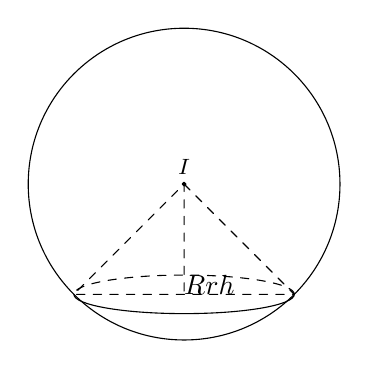
\begin{tikzpicture}[scale=0.7, font=\footnotesize, line join=round, line cap=round, >=stealth]
				\tikzset{label style/.style={font=\footnotesize}}
				\coordinate (A) at (2,0);
				\coordinate (I) at (0,2);
				\coordinate (K) at (0,0);
				\coordinate (B) at (-2,0);
				\draw[dashed] (A) arc (0:180:2cm and 0.35cm);
				\draw (A) arc (0:-180:2cm and 0.35cm);
				\draw (I) circle (2.828cm);
				\filldraw (I) node[above] {$I$} circle (1pt);
				%\filldraw (K) node[above right] {$K$} circle (1pt);
				%\filldraw (A) node[right] {$A$} circle (1pt);
				%\filldraw (B) node[left] {$B$} circle (1pt);
				\draw[dashed] (I)--(A)--(B)--(I)--(K);
				\tkzLabelSegment[above](I,A){$R$}
				\tkzLabelSegment[above=-0.1](K,A){$r$}
				\tkzLabelSegment[right](I,K){$h$}
			\end{tikzpicture}
		}
	}
\end{vd}
\dongcham{14}
\boxmini{BÀI TẬP TRẮC NGHIỆM}
\setcounter{ex}{0}
\Opensolutionfile{ans}[ans/2H5-B4-d3]
\begin{ex}
	Cho điểm $M\left(1;-1;3\right)$ và mặt cầu $(S)$ có phương trình$\left(x-1\right)^2+(y+2)^2+z^2=9$. Khẳng định đúng là
	\choice
	{\True $M$ nằm ngoài $(S)$}
	{$M$ nằm trong $(S)$}
	{$M$ nằm trên$(S)$}
	{$M$ trùng với tâm của $(S)$}
	\loigiai{
		Thay tọa độ $M$ vào vế trái của phương trình mặt cầu, ta được $(1-1)^2+(-1+2)^2+(3)^2=10>9$. Suy ra $M$ nằm ngoài $(S)$}
\end{ex}

\begin{ex}%[BG-12-New-4in1, Nguyễn Cường]%[2H5H3-3]
	Cho mặt cầu $(S)\colon x^2+y^2+z^2-2x-4y-6z = 0$ và ba điểm $O(0; 0; 0)$, $A(1; 2; 3)$, $B(2; -1; -1)$. Trong số ba điểm trên số điểm nằm trên mặt cầu là
	\choice
	{$2$}
	{$0$}
	{$3$}
	{\True $1$}
	\loigiai{Lần lượt thay tọa độ các điểm $O, A, B$ vào phương trình mặt cầu $(S)$ ta chỉ thấy duy nhất điểm $O$ thuộc mặt cầu $(S)$.
	}
\end{ex}

\begin{ex}%[BG-12-New-4in1, Nguyễn Cường]%[2H5H3-3]
	Cho mặt cầu $(S): x^2+y^2+z^2-4y+6z-2=0$ và mặt phẳng $(P)\colon x+y-z+4=0$. Trong các mệnh đề sau, mệnh đề nào đúng?
	\choice
	{ $(P)$ tiếp xúc $(S)$}
	{\True $(P)$ và $(S)$ không có điểm chung}
	{$(P)$ đi qua tâm của $(S)$}
	{$(P)$ cắt $(S)$}
	\loigiai{
		$(S)$ có tâm $I(0;2;-3)$ và bán kính $R=\sqrt{15}$.\\
		Ta có $\mathrm{d}[I,(P)]=\dfrac{\left|2+3+4 \right| }{\sqrt{1+1+1}}=3\sqrt{3} > \sqrt{15}=R$ nên $(P)$ và $(S)$ không có điểm chung.
	}
\end{ex}

\begin{ex}%[2H3B2-7]%Câu 9.
	Cho mặt phẳng $(P)$ và mặt cầu $(S)$ có phương trình lần lượt là $(P)\colon 2x+2y+z-m^2+4m-5=0$; $(S)\colon x^2+y^2+z^2-2x+2y-2z-6=0$. Giá trị của $m$ để $(P)$ tiếp xúc $(S)$ là
	\choice
	{$m=5$}
	{$m=-1$}
	{\True $m=-1$ hoặc $m=5$}
	{$m=1$ hoặc $m=-5$}
	\loigiai{
		Mặt cầu $(S)\colon x^2+y^2+z^2-2x+2y-2z-6=0$ có tâm $I(1;-1;1)$ và bán kính $R=3$.\\
		$(P)$ tiếp xúc $(S)\Leftrightarrow\mathrm{d}\left(I,(P)\right)=R$
		\begin{eqnarray*}
			&\Leftrightarrow&\dfrac{\left|2\cdot 1+2\cdot (-1)+1-m^2+4m-5\right|}{\sqrt{2^2+2^2+1^2}}=3\\
			&\Leftrightarrow&\left|m^2-4m+4\right|=9\\
			&\Leftrightarrow&\hoac{&m^2-4m+4=9\\&m^2-4m+4=-9\quad \text{(vô nghiệm)}}\\
			&\Leftrightarrow& m^2-4m-5=0\Leftrightarrow\hoac{&m=-1\\&m=5.}
		\end{eqnarray*}
	}
\end{ex}

\begin{ex}%[Thi thử L3, Yên Lạc 2, Vĩnh Phúc 2018]%[Hoàng Trình,12EX6]%[2H3B2-7]%
	Trong không gian với hệ tọa độ $Oxyz$, cho mặt phẳng $(P)\colon 2x+2y+z-2=0$ và mặt cầu $(S)$ tâm $I\left(2;1;-1\right)$ bán kính $R=2$. Bán kính đường tròn giao của mặt phẳng $(P)$ và mặt cầu $(S)$ là
	\choice
	{\True $r=\sqrt{3}$}
	{$r=\sqrt{5}$}
	{$r=1$}
	{$r=3$}
	\loigiai{
		\immini{
			Gọi bán kính đường tròn giao của mặt phẳng $(P)$\\
			và mặt cầu $(S)$ là $r$.\\
			Ta có $h=\mathrm{d}(I,(P))=\dfrac{\left|2\cdot 2+2\cdot (-1)-1-2 \right| }{\sqrt{2^2+2^2+1^2}}=1$.\\
			Suy ra $r=\sqrt{2^2-1^2}=\sqrt{3}$.
		}
		{
			\begin{tikzpicture}[line width=0.6pt]
				\draw[fill=black] (0,0)coordinate(I) circle(1pt) node[above left]{$I$};
				\draw[fill=black] (0,-0.9)coordinate(H) circle(1pt);
				\node at (0,-0.9) [left]{$H$};
				\draw[dashed] (0,0)--(0,-0.9)--(1,-1.3)coordinate(M)--(0,0);
				\tkzMarkRightAngle(I,H,M)
				\node at (0.83,-0.7) {$R$};
				\node at (0.4,-1.23) {$r$};
				\draw[line width=0.6pt] (1.61,-1.01) arc [radius=1.9, start angle=-32.1, end angle=212];
				\draw[line width=0.6pt] (-1.164,-1.5) arc [radius=1.9, start angle=-127.9, end angle=-52];
				\draw[dashed,line width=0.6pt] (-1.61,-1.01) arc [radius=1.9, start angle=212, end angle=232.1];
				\draw[dashed,line width=0.6pt] (1.61,-1.01) arc [radius=1.9, start angle=-32.1, end angle=-52];
				\coordinate (A) at (-2.7,-1.5);
				\coordinate (B) at (-1.7,-0.3);
				\coordinate (C) at (2.6,-0.3);
				\coordinate (D) at ($(A)+(C)-(B)$);
				\draw (-1.84,-0.47)--(A)--(D)--(C)--(1.87,-0.3);
				\draw[line width=0.5pt,dashed] (-1.84,-0.47)--(B)--(1.87,-0.3);
				\draw[dashed] (-1.64,-0.9)..controls (-1.57,-0.2) and (1.57,-0.2)..(1.64,-0.9);
				\draw (-1.64,-0.9)..controls (-1.57,-1.6) and (1.57,-1.6)..(1.64,-0.9);
				\node at (-2.25,-1.3) {$(P)$};
				\node at (-1.9,1.3) {$(S)$};
				\draw (-2.1,-1.5)..controls (-1.95,-1.1)..(-2.34,-1.05);
			\end{tikzpicture}
		}
	}
\end{ex}

\begin{ex}%[Dự án EX-7-2019]%[Phạm Tuấn]%[2H3B2-7]%
	Trong không gian $Oxyz $, mặt cầu có phương trình $x^2+y^2+z^2-2x+2y-6z+2=0$
	cắt mặt phẳng $(Oxz)$ theo một đường tròn có bán kính bằng
	\choice
	{$3\sqrt{2}$}
	{\True $2\sqrt{2}$}
	{$5$}
	{$4\sqrt{2}$}
	\loigiai{
		Mặt cầu đã cho có tâm $I(1;-1;3)$ và bán kính $R=3$. \\
		Khoảng cách từ $I$ đến mặt phẳng $(Oxz)$ bằng $1$, do đó bán kính của đường tròn bằng \[\sqrt{3^2-1^2}=2\sqrt{2}.\]
	}
\end{ex}

\begin{ex}%[Thi thử L1, Chuyên Ngoại Ngữ, Hà Nội, 2018]%[2H3B2-7]%[Nguyễn Bình Nguyên-12Ex8]%
	Trong không gian với hệ trục tọa độ $Oxyz$, cho mặt cầu $(S) \colon (x-1)^2+(y-2)^2+(z-2)^2=9$ và mặt phẳng $(P) \colon 2x-y-2z+1=0$. Biết $(P)$ cắt $(S)$ theo giao tuyến là đường tròn có bán kính $r$. Tính $r$.
	\choice
	{$r=3$}
	{$r=2$}
	{\True $r=2\sqrt{2}$}
	{$r=\sqrt{3}$}
	\loigiai
	{Ta có $(S) \colon (x-1)^2+(y-2)^2+(z-2)^2=9$ $\Rightarrow \heva{&I(1;2;2)\\&R=3}.$\\ $d=\mathrm{d}\left(I,(\alpha)\right)=\dfrac{|2\cdot1-2-2\cdot2+1|}{\sqrt{2^2+(-1)^2+(-2)^2}}=1.$\\
		Vậy	$r=\sqrt{R^2-d^2}=2\sqrt{2}$.}
\end{ex}

\begin{ex}%[Thi thử L2, Lương Thế Vinh, Hà Nội, 2018]%[Phạm Toàn, Dự án (12EX-9)]%[2H3B2-7]%
	Trong không gian $Oxyz$ cho mặt cầu $(S)\colon x^2+y^2+z^2-6x-4y-12z=0$ và mặt phẳng $(P)\colon 2x+y-z-2=0$. Tính diện tích thiết diện của mặt cầu $(S)$ cắt bởi mặt phẳng $(P)$.
	\choice
	{$50\pi $}
	{\True $S=49\pi $}
	{$25\pi $}
	{$36\pi $}
	\loigiai{
		Mặt cầu $(S)$ có tâm $I(3;2;6)$ và bán kính $R=\sqrt{3^2+2^2+6^2}=7$. Vì $I$ thuộc $(P)$ nên $(P)$ cắt $(S)$ theo thiết diện là đường tròn có bán kính bằng $7$. Diện tích thiết diện bằng $49\pi$.
	}
\end{ex}

\begin{ex}%[Đề thi thử Tốt nghiệp THPT lần 1, Sở GD&ĐT Hà Nội, 2020]%[Nguyễn Đắc Giáp, 12EX8]%[2H3B2-7]%
	Trong không gian với hệ tọa độ $Oxyz$, cho điểm $I(2;1;1)$ và mặt phẳng $(P)\colon 2x+y+2z-1=0$. Mặt cầu $(S)$ có tâm $I$, cắt $(P)$ theo một đường tròn có bán kính $r=4$. Mặt cầu $(S)$ có phương trình là
	\choice
	{$(x-2)^2 + (y-1)^2 + (z-1)^2 =18$}
	{$(x-2)^2 + (y-1)^2 +(z-1)^2 = 2\sqrt{5}$}
	{\True $(x-2)^2 + (y-1)^2 + (z-1)^2 =20$}
	{$(x+2)^2 + (y+1)^2 + (z+1)^2 =20$}
	\loigiai{
		Ta có $$\mathrm{d}(I;(P)) = \dfrac{\left | 2\cdot 2+1+2\cdot 1-1  \right |}{\sqrt{2^2+1^2+2^2}} =2.$$
		Vì mặt cầu $(S)$ có tâm $I$, cắt $(P)$ theo một đường tròn có bán kính $r=4$ nên mặt cầu $(S)$ có bán kính
		$$R=\sqrt{r^2+\mathrm{d}^2(I,(P))} = \sqrt{4^2+2^2} = 2\sqrt{5}.$$
		Vậy phương trình mặt cầu $(S)$ là $(x-2)^2 + (y-1)^2 + (z-1)^2 =20$.
	}
\end{ex}

\begin{ex}%[HK2, Sở GD&ĐT Đà Nẵng, 2019]%[Trần Chiến, 12EX6-2020]%[2H3B2-7]%
	Trong không gian $Oxyz$, cho mặt cầu $(S)$ có tâm $I(1;2;1)$ và cắt mặt phẳng $(P)\colon 2x-y+2z+7 =0$ theo một đường tròn có đường kính bằng $8$. Phương trình mặt cầu $(S)$ là
	\choice
	{\True $(x-1)^2+(y-2)^2 +(z-1)^2=25$}
	{$(x-1)^2+(y-2)^2 +(z-1)^2=81$}
	{$(x+1)^2+(y+2)^2 +(z+1)^2=9$}
	{$(x-1)^2+(y-2)^2 +(z-1)^2=5$}
	\loigiai{
		\immini{
			Gọi $R$, $r$, $d$ lần lượt là bán kính của mặt cầu, bán kính của đường tròn và khoảng cách từ tâm $I$ đến mp$(P)$. Khi đó $R = \sqrt{r^2+d^2}$.\\
			Ta có $d= \mathrm{d}(I,(P)) =\dfrac{|2\cdot 1 -2+2\cdot 1+7|}{\sqrt{2^2+ (-1)^2+2^2}} = 3$ và $r=4$. \\
			Suy ra $R =\sqrt{3^2+4^2}=5$.\\
			Vậy phương trình mặt cầu $(S)$ là $(x-1)^2+(y-2)^2 +(z-1)^2=25$.
		}{
			\begin{tikzpicture}[scale=0.7, font=\footnotesize, line join=round, line cap=round, >=stealth]
				\tkzDefPoints{0/0/O}
				\def\a{3}
				\def\b{0.6}
				\coordinate (M) at (0:\a cm and \b cm);
				\coordinate (I) at ($(O)+(0,1.5)$);
				\tkzDrawCircle(I,M)
				\draw (M) arc (0:-180:\a cm and \b cm);
				\draw[dashed] (M) arc (0:180:\a cm and \b cm);
				\tkzDrawSegments[dashed](I,O I,M M,O)
				\tkzDrawPoints[fill=black](I,O,M)
				\tkzLabelSegment[left](I,O){$d$}
				\tkzLabelSegment[above right](I,M){$R$}
				\tkzLabelSegment[below](M,O){$r$}
			\end{tikzpicture}
		}
	}
\end{ex}
\Closesolutionfile{ans}

